\section{Auswertung}
\label{sec:Auswertung}

\begin{table}
    \centering
    \begin{tabular}{
    S[table-format=3.0]
    S[table-format=1.2]
    S[table-format=1.2]
  }
    \toprule
    {Phase\;$\phi \left[\unit{°}\right]$} & {$U_{out}\left[\unit{V}\right]$} & {$U_{out noise}\left[\unit{V}\right]$}\\
    \midrule
    000 & 0.00  & 0.00 \\
    030 & 2.08  & 2.02 \\
    060 & 4.60  & 4.53 \\
    090 & 5.15  & 5.00 \\
    120 & 4.75  & 4.60 \\
    150 & 2.43  & 2.18 \\
    180 & 0.00  & 0.00 \\ 
    210 & -2.03 & -1.80  \\
    240 & -4.80 & -4.30  \\
    270 & -5.40 & -4.85  \\
    300 & -4.98 & -4.40  \\
    330 & -2.40 & -2.01  \\
    360 & 0.00  & 0.00 \\
    \bottomrule
\end{tabular}
\end{table}
In den Abbildungen 5 bis 9 sind Screenshots von der Anzeige des Oszilloskops für die verschiedenen Phasen $\phi$ dargestellt. In Abbildung 10 ist
die Anzeige bei Phase $\phi = 0$, jedoch mit aktiviertem Noise, dargestellt. Durch den Rauschgenerator ist das Signal nicht mehr sinusförmig. Ein Signal wäre nicht mehr verwendbar in diesem Zustand.\\
\begin{figure}
    \begin{minipage}[b]{.45\linewidth} % [b] => Ausrichtung an \caption
       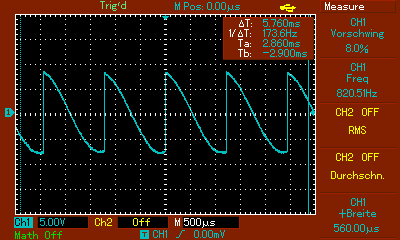
\includegraphics[width=\linewidth]{bilder/MAP003.png}
       \caption{$\phi = 0\,\unit{°}$}
    \end{minipage}
    \hspace{0.1\linewidth}% Abstand zwischen Bilder
    \begin{minipage}[b]{.45\linewidth} % [b] => Ausrichtung an \caption
       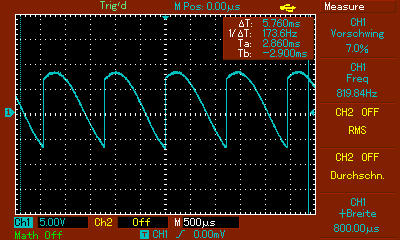
\includegraphics[width=\linewidth]{bilder/MAP004.png}
       \caption{$\phi = 30\,\unit{°}$}
    \end{minipage}
\end{figure}

\begin{figure}
    \begin{minipage}[b]{.45\linewidth} % [b] => Ausrichtung an \caption
       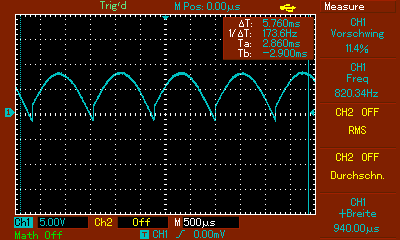
\includegraphics[width=\linewidth]{bilder/MAP005.png}
       \caption{$\phi = 60\,\unit{°}$}
    \end{minipage}
    \hspace{0.1\linewidth}% Abstand zwischen Bilder
    \begin{minipage}[b]{.45\linewidth} % [b] => Ausrichtung an \caption
       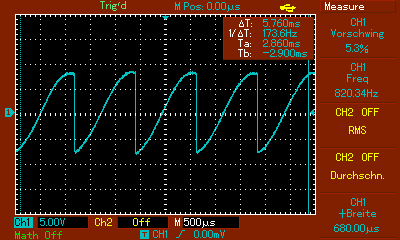
\includegraphics[width=\linewidth]{bilder/MAP006.png}
       \caption{$\phi = 90\,\unit{°}$}
    \end{minipage}
\end{figure}

\begin{figure}[h]
    \begin{minipage}[b]{.45\linewidth} % [b] => Ausrichtung an \caption
       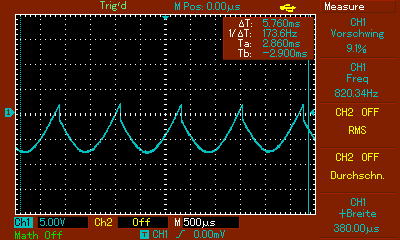
\includegraphics[width=\linewidth]{bilder/MAP007.png}
       \caption{$\phi = 120\,\unit{°}$}
    \end{minipage}
    \hspace{0.1\linewidth}% Abstand zwischen Bilder
    \begin{minipage}[b]{.45\linewidth} % [b] => Ausrichtung an \caption
       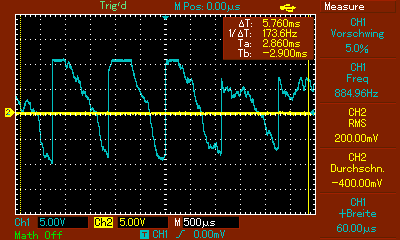
\includegraphics[width=\linewidth]{bilder/MAP011.png}
       \caption{$\phi = 0\,\unit{°}$ mit Noise}
    \end{minipage}
\end{figure}

%Plots
\begin{figure}[H]
    \begin{minipage}[b]{.49\linewidth} % [b] => Ausrichtung an \caption
       \includegraphics[width=\linewidth]{build/U_out.pdf}
       \caption{$U_{out}$ ohne Noise}
       \label{fig:FitU}
    \end{minipage}
    \hspace{0.02\linewidth}% Abstand zwischen Bilder
    \begin{minipage}[b]{.49\linewidth} % [b] => Ausrichtung an \caption
       \includegraphics[width=\linewidth]{build/U_outnoise.pdf}
       \caption{$U_{out}$ mit Noise}
       \label{fig:FitU_noise}
    \end{minipage}
\end{figure}
Der Lock-In-Verstärker filtert das vom Rauschgenerator erzeugte Störsignal effektiv heraus. Die Spannung ist proportional zur Phase.
Die Fitfunktion in Abbildung \ref{fig:FitU} ist
\begin{equation*}
   U_{out}(\phi) = a \cdot \sin(b\cdot\phi + c) + d
\end{equation*}
mit den Parametern
\begin{equation*}
   a = (5.282 \pm 0.132) \,\unit{V}, \quad b = (1.006 \pm 0.010) \,, \quad c = (-2.416 \pm 2.313) \,, \quad d = (-0.037 \pm 0.089) \,\unit{V}.
\end{equation*}
Für den Fit in der Abbildung \ref{fig:FitU_noise} wurde die selbe Funktion verwendet mit den Parametern
\begin{equation*}
   a = (4.901 \pm 0.136) \,\unit{V}, \quad b = (1.008 \pm 0.011) \,, \quad c = (-2.253 \pm 2.559) \,, \quad d = (0.080 \pm 0.091) \,\unit{V}.
\end{equation*}
\begin{figure}
    \centering
    \includegraphics[width=\linewidth]{build/diode1.pdf}
    \caption{$U$ in Abhängigkeit des Abstands $r$}
\end{figure}
Die Spannung ist antiproportional zum Abstand. Selbst bei einem großen Abstand ist das Signal der LED noch vom Hintergrundrauschen unterscheidbar.
Für den Fit wurde die Funktion 
\begin{equation*}
   U_{out}(\phi) = \frac{a}{r^b} + c
\end{equation*}
verwendet, mit den Parametern
\begin{equation*}
   a = (5846.649 \pm 772.499) \,\unit{\V\per\centi\m} , \quad b = (3.117 \pm 0.056) \, , \quad c = (0.032 \pm 0.010) \,\unit{V}.
\end{equation*}

\newpage